% !TeX program = xelatex
\documentclass[UTF8,a4paper,10pt,twocolumn,fontset=none]{ctexart}

\usepackage{iftex}
\ifXeTeX\else
  \PackageError{market-report}{This document must be compiled with XeLaTeX}
  {In Overleaf, open Menu -> Settings -> Compiler and select XeLaTeX.}
\fi
\setCJKmainfont{FandolSong-Regular}
\setCJKsansfont{FandolHei-Regular}
\setCJKmonofont{FandolFang-Regular}

\usepackage[left=1.50cm,right=1.50cm,top=1.50cm,bottom=1.55cm,columnsep=0.68cm]{geometry}
\usepackage{amsmath,amssymb,booktabs,tabularx,array,multirow}
\usepackage{graphicx,subcaption,float,enumitem,hyperref,xcolor,microtype}
\usepackage[section]{placeins}
\usepackage{tikz}
\usetikzlibrary{arrows.meta,positioning,shapes.geometric}

\hypersetup{
  colorlinks=true,
  linkcolor=black,
  citecolor=blue!55!black,
  urlcolor=blue!55!black
}
\setlength{\parindent}{2em}
\setlength{\parskip}{0pt}
\setlength{\columnsep}{0.68cm}
\setlength{\floatsep}{7pt plus 2pt minus 1pt}
\setlength{\textfloatsep}{8pt plus 2pt minus 2pt}
\setlength{\intextsep}{7pt plus 2pt minus 1pt}
\setlength{\abovecaptionskip}{3pt}
\setlength{\belowcaptionskip}{0pt}
\setlist{nosep,leftmargin=1.45em}
\renewcommand{\baselinestretch}{1.06}
\newcolumntype{Y}{>{\raggedright\arraybackslash}X}
\pagestyle{plain}

\ctexset{
  section={format=\large\bfseries,beforeskip=5pt,afterskip=2pt},
  subsection={format=\normalsize\bfseries,beforeskip=3pt,afterskip=1pt}
}
\captionsetup{font=small,labelfont=bf}

\title{\vspace{-1.2cm}\textbf{基于金融新闻情绪与股票价格数据的市场趋势预测研究}}
\author{黄文轩\quad 王子轩\quad 林瀚羽\quad 彭琰轲\\
\small 深圳大学金融科技专业}
\date{}

\begin{document}

\maketitle
\vspace{-1.7em}
\begin{abstract}
\small
金融市场会对新闻中的新增信息与投资者预期作出反应，但新闻情绪是否具有稳定的
样本外预测价值仍存在争议。本文基于Combined News and DJIA公开数据，将2008年
8月至2016年7月每日25条新闻标题与道琼斯工业平均指数（DJIA）行情匹配。为避免
同日新闻与收盘价之间的时点歧义，使用$t$日新闻情绪和截至$t$日可观测的量价指标，
预测$t+1$日指数方向。本文以VADER提取情绪，构造情绪均值、分歧、正负占比和
滞后变化等变量，比较Logistic回归、随机森林与XGBoost在“仅量价”和
“量价+新闻”两组特征下的表现。2014--2016年walk-forward实验表明，XGBoost加入
新闻后平均ROC-AUC由0.472提高至0.504，但AUC增量的95\% bootstrap置信区间为
$[-0.006,0.073]$，未达到统计显著。新闻策略扣除10个基点仓位调整成本后的年化
收益为$-13.1\%$，夏普比率为$-1.51$。年度稳定性、相关性、概率校准和阈值敏感性
分析进一步显示，新闻情绪至多提供微弱且时变的非线性信息，尚不足以支持稳定交易。

\noindent\textbf{关键词：}金融新闻；情绪分析；VADER；股票趋势预测；XGBoost；
walk-forward验证
\end{abstract}
\vspace{0.4em}

\section{引言}

股票市场具有高度信息驱动特征。传统预测通常使用收益率、成交量、移动平均线和
波动率等结构化变量，但公司事件、宏观政策、地缘冲突和媒体叙事也会改变投资者预期。
Tetlock发现媒体悲观语调与市场收益及交易量存在关系\cite{tetlock}；
Loughran和McDonald进一步表明，通用情感词典会误判大量金融术语，领域语境不可
忽略\cite{lm}。

近年来，文本预测研究从词典计数发展到事件表示、神经网络和预训练语言模型。
Ding等将新闻事件转换为稠密表示并用于指数预测\cite{ding2015}；StockNet联合
社交文本与历史价格建模\cite{stocknet}；FinBERT通过金融语料适配提升金融情绪
分类能力\cite{finbert}；FNSPID和CausalStock则进一步面向大规模、多股票和关系
建模\cite{fnspid,causalstock}。这些工作说明新闻与价格融合具有研究价值，但也
意味着预测效果高度依赖数据规模、时间戳质量、文本与公司的匹配粒度。

公开教学数据常只有每日新闻标题而没有精确发布时间。若直接用当天全部标题预测
当天收盘标签，模型可能读取收盘后新闻；若随机拆分时间序列，未来市场状态会进入
训练集。为降低这两类偏差，本文将任务重新定义为严格的下一交易日预测，并采用
递增窗口和隔离期。

本文贡献包括：（1）构造新闻情绪与量价特征的可复现实验管线；（2）以特征消融
直接检验新闻的增量价值；（3）同时报告统计显著性、年度稳定性、概率校准和经济
回测；（4）如实分析接近随机和回测失败的结果，避免只展示表现最好的窗口。

\subsection{研究问题与现实意义}

从应用角度看，新闻情绪预测并不只是追求分类准确率。智能投研系统需要回答的是：
新增文本信息能否在既有量价信号之外提供边际价值，模型给出的概率是否可信，以及
这种概率能否覆盖交易成本。若模型仅在随机划分下取得较高准确率，却不能在后续年份
复现，其结果无法支持真实决策。因此本文将研究目标分解为三个层次：首先检验新闻
特征是否改善统计排序；其次检验改善是否跨年份稳定；最后检验信号是否具有经济价值。

从课程大数据分析角度看，本研究同时涉及非结构化文本、结构化时序数据、异构数据
对齐、监督学习和模型评价。新闻标题需要经过清洗和情绪量化，行情数据需要计算滚动
指标，两类数据还必须按交易日对齐。该过程比单独训练一个分类器更能体现完整的数据
分析链路。

\subsection{新闻影响市场的可能机制}

新闻影响价格至少存在三条路径。第一是\textbf{基本面信息渠道}，例如盈利、并购和
政策变化会修正未来现金流预期。第二是\textbf{风险偏好渠道}，战争、危机和宏观不确定
性可能提高投资者要求的风险补偿。第三是\textbf{注意力渠道}，高热度新闻会改变交易者
关注度、成交量和短期资金流。理论上，若市场不能瞬时吸收这些信息，$t$日新闻就可能
对$t+1$日收益产生预测作用；若市场接近半强式有效，公开标题的信息会快速进入价格，
下一日可预测性便会很弱。本文结果实际上是对这两种观点的样本外检验。

\begin{figure}[!htbp]
\centering
\begin{tikzpicture}[
  node distance=0.20cm,
  box/.style={draw,rounded corners,align=center,minimum height=1.0cm,
              text width=3.15cm,fill=blue!5,font=\footnotesize},
  arrow/.style={-{Latex[length=2mm]},thick}
]
\node[box] (news) {每日Top 25新闻\\文本清洗与VADER};
\node[box,below=of news] (sent) {日度情绪特征\\均值、分歧、正负占比};
\node[box,below=of sent] (price) {DJIA行情特征\\收益、波动、量价指标};
\node[box,below=of price] (panel) {时间对齐面板\\$t$日特征预测$t+1$};
\node[box,below=of panel] (model) {LR / RF / XGBoost\\P与P+N消融};
\node[box,below=of model] (eval) {walk-forward\\统计检验与回测};
\draw[arrow] (news)--(sent);
\draw[arrow] (sent)--(price);
\draw[arrow] (price)--(panel);
\draw[arrow] (panel)--(model);
\draw[arrow] (model)--(eval);
\end{tikzpicture}
\caption{本文的数据处理、建模与验证流程}
\label{fig:workflow}
\end{figure}

\section{文献综述}

\subsection{词典、情绪分类与金融语义}

早期金融文本研究多使用正负词频。Tetlock以媒体悲观词比例刻画市场情绪
\cite{tetlock}。Loughran--McDonald词典针对公司报告构建金融类别词汇，揭示
“liability”等词在一般语境与金融语境中的极性差异\cite{lm}。Financial
PhraseBank由金融专业人员标注句子情绪，是金融情绪分类常用基准\cite{phrasebank}。

VADER综合词典、否定、程度副词、大小写和标点规则，输出$[-1,1]$的compound
分数\cite{vader}。其优点是透明、无需训练且可完整复现，缺点是缺少金融领域
适配。FinBERT通过在金融语料上继续预训练并微调情绪分类，能更好处理上下文和
金融术语\cite{finbert}。本文选择VADER作为低成本基线，并将领域模型作为后续扩展。

\subsection{新闻驱动的市场预测}

Ding等使用事件抽取和深度卷积网络预测S\&P 500方向，强调事件结构比词袋更能表达
“谁对谁做了什么”\cite{ding2015}。StockNet将推文、用户信息与价格序列联合输入
变分循环模型，说明文本信号与价格动态可能存在时变交互\cite{stocknet}。
Akita等将新闻段落向量与股票价格结合，发现融合模型可能优于单一模态，但结果依赖
样本和市场\cite{akita}.

更近期研究转向大规模和关系建模。FNSPID整合千万级新闻与数千只股票价格，为
时间序列新闻研究提供更大数据基础\cite{fnspid}。CausalStock尝试从新闻和股票
关系中学习因果结构\cite{causalstock}。与这些数据相比，本文数据只有约2000个
交易日、且新闻是全球热点而非公司级事件，因此预期效果应更保守。

\subsection{现有研究的评价差异}

已有论文的结论并不能直接横向比较。一方面，研究对象可能是市场指数、单只股票或
横截面股票组合；另一方面，标签可能是同日方向、下一日方向、收益率回归或超额收益。
文本来源也包括新闻全文、标题、推文和公司公告。若使用新闻全文和精确时间戳，模型
能够获得比每日汇总标题更多的信息；若使用同日标签，则可能混入时间顺序不清的问题。

评价方式同样会改变结论。准确率受类别比例影响，AUC只衡量排序而不衡量概率校准，
回测收益又受阈值、交易成本和持仓规则影响。部分工作只报告单次测试结果，难以判断
模型是否依赖特定市场阶段。基于这些差异，本文不追求与文献中的最高准确率直接比较，
而强调同一数据和同一验证窗口下P与P+N的配对比较。

\subsection{研究假设}

\textbf{H1：}P+N模型的样本外AUC高于同算法P模型。\\
\textbf{H2：}新闻增量在不同测试年份保持同方向。\\
\textbf{H3：}若概率信号有效，扣除成本后应优于持有现金，并具有合理校准。

\section{数据与变量}

\subsection{数据来源与样本}

数据来自Kaggle的Daily News for Stock Market Prediction及公开镜像
\cite{dataset}。新闻表含\texttt{Date}和\texttt{Top1--Top25}；行情表含
DJIA开盘价、最高价、最低价、收盘价、成交量和复权收盘价。原始新闻表有1989日。
合并行情、构造20日滚动变量并删除末日无标签记录后，最终样本为1968日、
49193条有效标题，覆盖2008年9月8日至2016年6月30日。

该数据集每天保留Reddit世界新闻板块中排名较高的25条标题，能够近似反映当日公众
关注的宏观信息环境。其优势是日期覆盖连续、字段简单且容易复现；缺点是新闻主题
不一定与DJIA成分公司直接相关，也没有来源、精确发布时间和公司代码。由于这些限制，
本文将其定位为“市场级新闻情绪基线数据”，而不是公司级事件数据库。

\begin{table}[t]
\centering
\caption{样本描述统计}
\small
\begin{tabular}{lr}
\toprule
指标 & 数值\\
\midrule
交易日样本 & 1,968\\
有效新闻标题 & 49,193\\
平均每日标题数 & 25.00\\
下一日上涨比例 & 53.51\%\\
上涨日前情绪均值 & $-0.2150$\\
下跌日前情绪均值 & $-0.2168$\\
测试期样本数 & 575\\
\bottomrule
\end{tabular}
\label{tab:sample}
\end{table}

\subsection{数据质量检查}

预处理阶段按日期升序检查新闻表和行情表，去除重复日期，并确认合并后的交易日唯一。
标题字段中的\texttt{b'}前缀来自早期Python字节串保存格式，若不清除会被情绪模型
当作普通字符。本文同时替换HTML实体、异常引号和连续空格。少数标题数不足25条的
日期仍按有效标题数量计算平均值，避免人为补充文本。

行情侧使用复权收盘价计算收益，降低指数调整带来的不连续影响。成交量为零或滚动
窗口不足产生的无穷值和缺失值先转换为缺失状态，再由每个训练窗口的中位数填补。
测试期不参与填补统计量计算。最终上涨比例为53.51\%，虽然并非严重不平衡，但始终
预测上涨就能获得较高召回率和表面F1，因此必须结合AUC和平衡准确率判断。

\subsection{新闻清洗与情绪特征}

清除Python字节串前缀、异常引号、HTML实体和多余空白。对第$t$日第$j$条标题
计算VADER分数$s_{j,t}$，日均情绪定义为：
\begin{equation}
\bar{s}_t=\frac{1}{N_t}\sum_{j=1}^{N_t}s_{j,t}.
\end{equation}
进一步构造情绪标准差、最小值、最大值、正向占比、负向占比、中性占比、滞后情绪
与情绪变化。VADER阈值采用官方常见规则：$s\geq0.05$为正向，
$s\leq-0.05$为负向。

各情绪变量具有不同含义。日均情绪反映整体语调；情绪标准差刻画同日新闻之间的意见
分歧；最小值用于捕捉极端负面事件；正负占比能够避免少量高绝对值标题完全支配均值；
滞后情绪和情绪变化则分别表示情绪持续性与边际冲击。由于新闻排名可能代表注意力，
更理想的扩展方案还可对Top1--Top5赋予更高权重，但本研究保持等权以减少人为设定。

\begin{figure}[t]
\centering
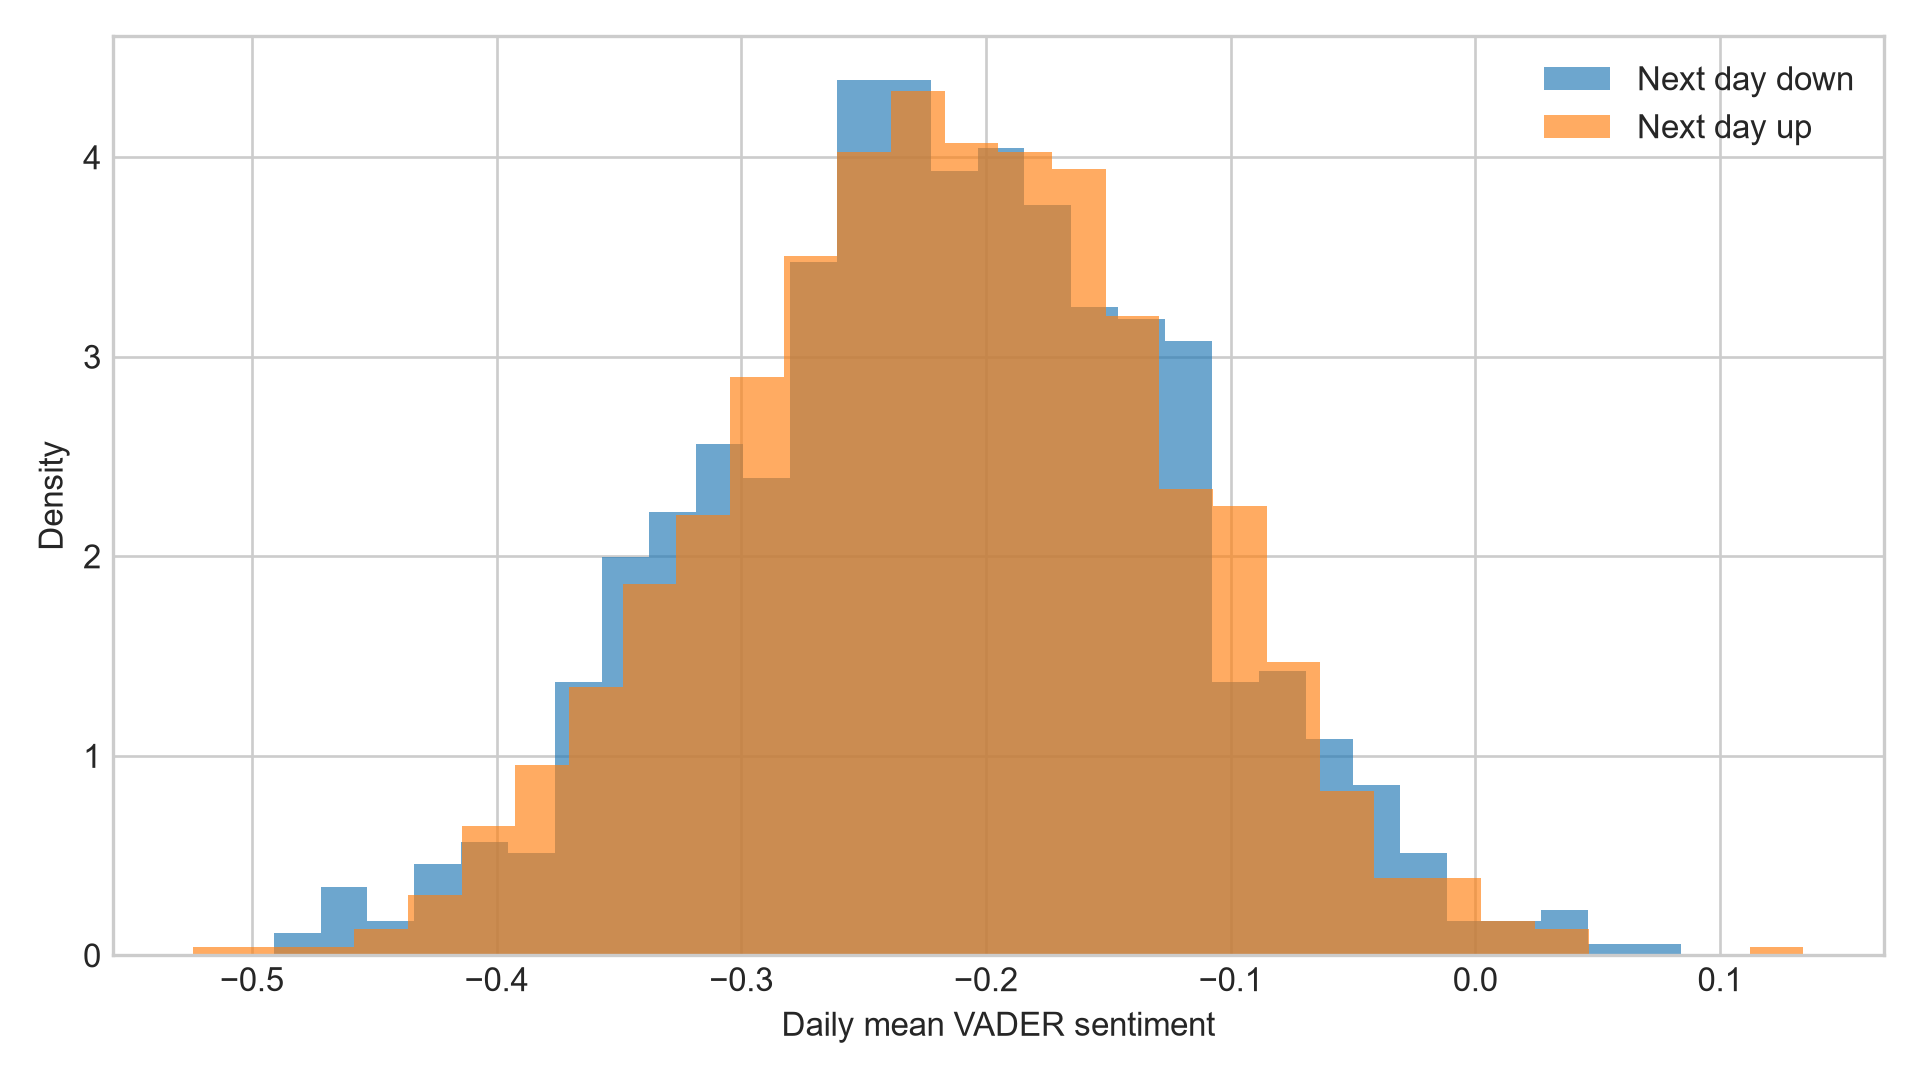
\includegraphics[width=\columnwidth]{figures/sentiment_distribution.png}
\caption{下一日上涨与下跌样本的日均新闻情绪分布}
\label{fig:sentdist}
\end{figure}

图\ref{fig:sentdist}显示两组分布高度重合。上涨日前与下跌日前平均情绪仅相差
0.0018，说明简单情绪均值难以形成线性可分信号。

\subsection{量价特征与标签}

以复权收盘价$P_t$计算$k$日收益率：
\begin{equation}
r_t^{(k)}=P_t/P_{t-k}-1.
\end{equation}
价格特征包括1/5/10/20日收益、5/20日均线差、5日和20日实现波动率、成交量变化、
日内振幅与5日动量方向。预测标签为：
\begin{equation}
y_{t+1}=\mathbb{I}(P_{t+1}/P_t-1>0).
\end{equation}
原数据同日标签不用于主实验。图\ref{fig:corr}中，日均情绪与下一日收益的相关系数
约为0.00，负面新闻占比约为$-0.04$；历史1日和5日收益与下一日收益均约为$-0.10$。

均线差描述短期价格相对中期趋势的位置，波动率反映近期风险状态，成交量变化表示
市场参与程度，日内振幅则近似刻画当日信息冲击。选择这些变量的目的不是建立完整
技术交易系统，而是形成一个具有合理解释力的量价基线。只有当新闻模型超过这一
基线时，才能说明文本信息具有独立贡献。

\begin{figure}[t]
\centering
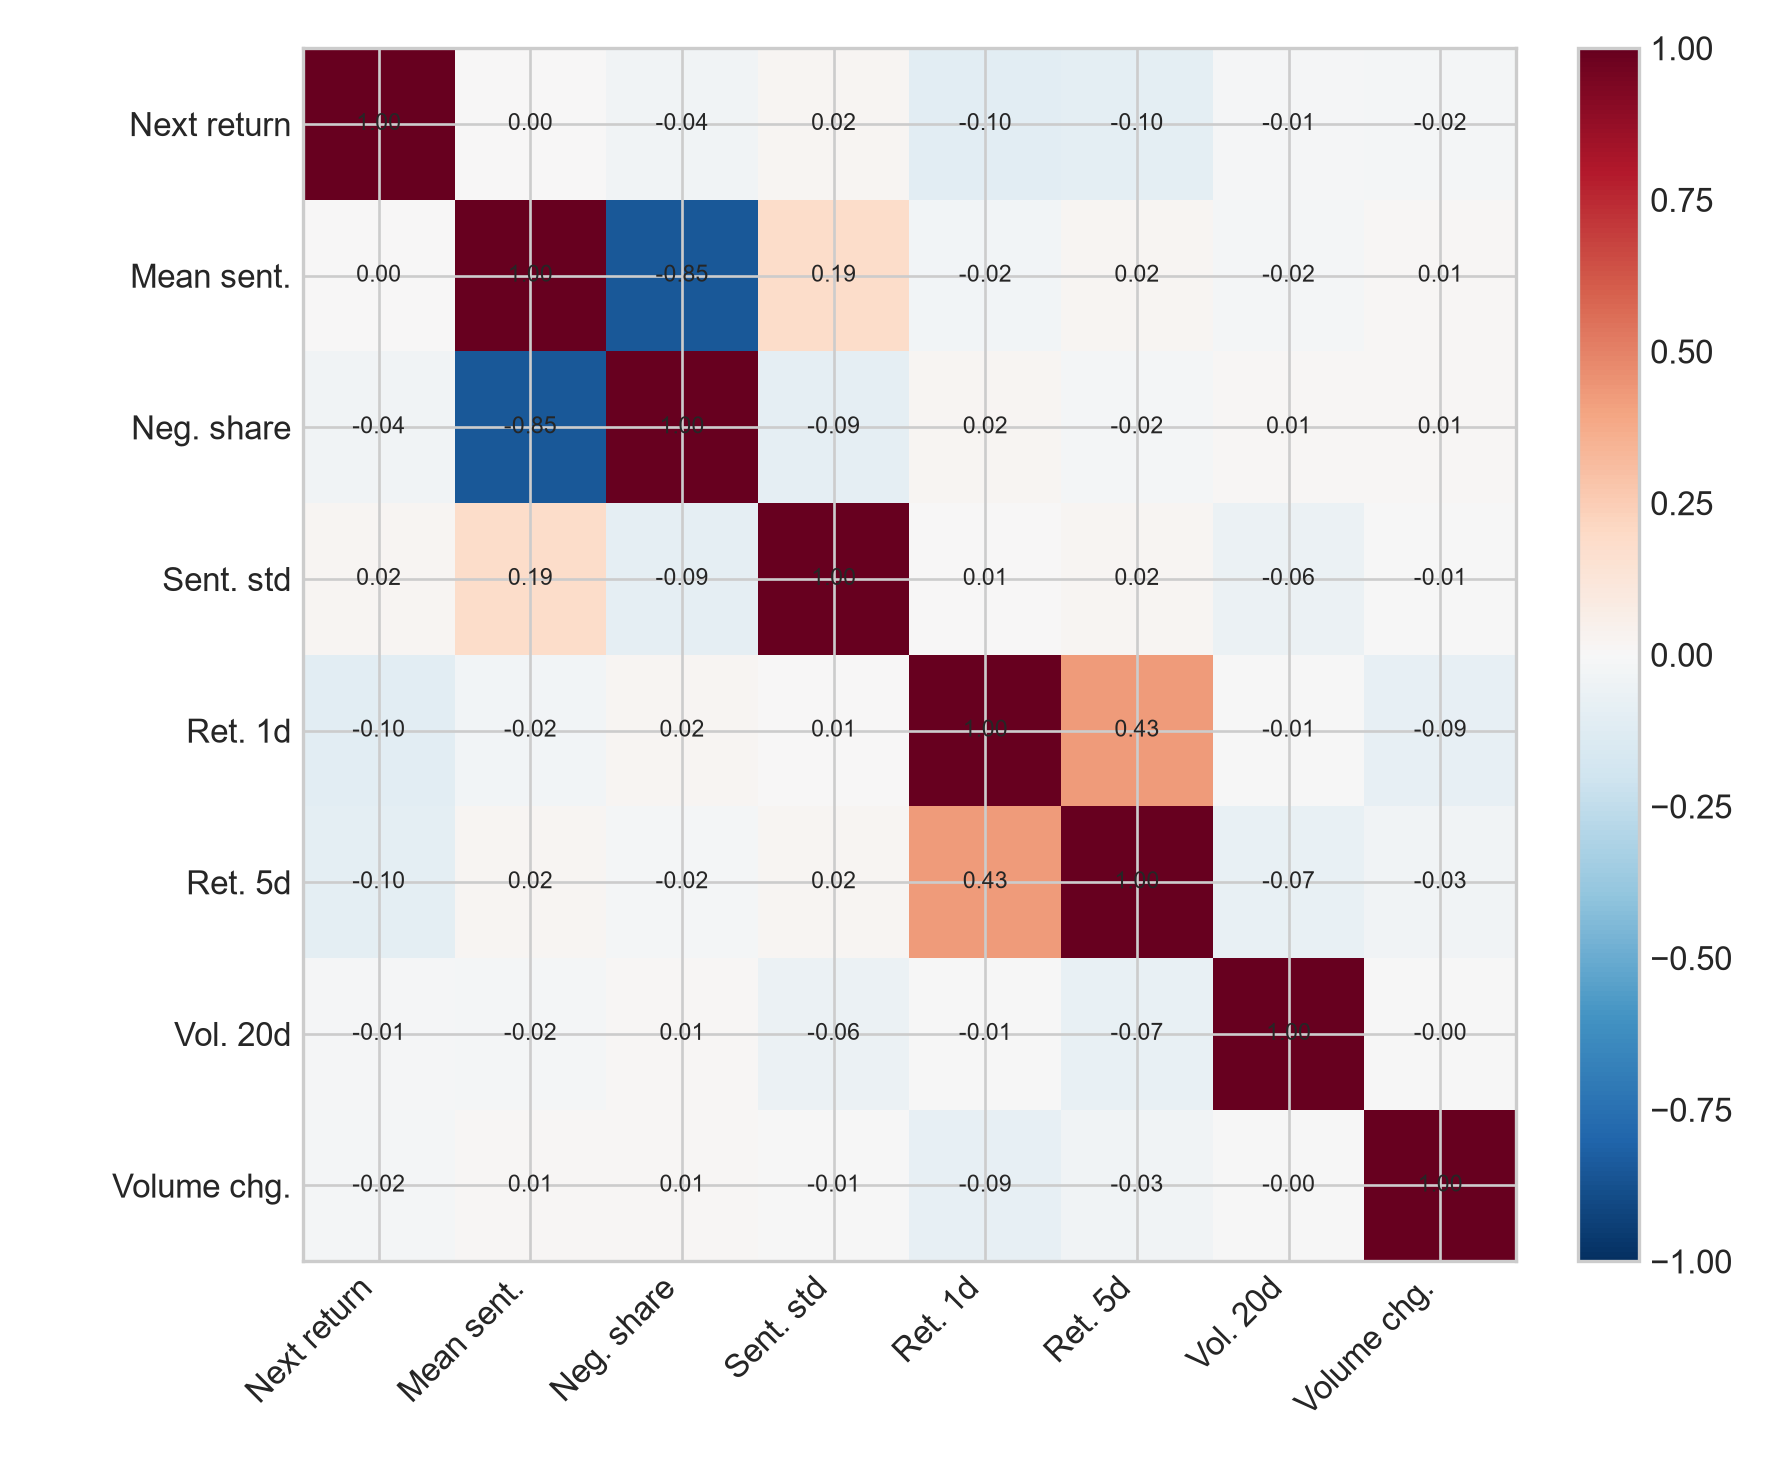
\includegraphics[width=\columnwidth]{figures/feature_correlation.png}
\caption{主要新闻、量价变量与下一日收益的相关系数}
\label{fig:corr}
\end{figure}

\section{研究方法}

\subsection{模型与特征消融}

Logistic回归作为线性基准并设置类别权重；随机森林使用500棵树、最大深度5和
最小叶节点12；XGBoost使用350棵深度3的树、学习率0.025、0.8行列采样以及
$L_1/L_2$正则化\cite{xgboost}。设置：
\begin{itemize}
  \item P：仅量价和技术指标；
  \item P+N：P加新闻情绪、占比、分歧和滞后变量。
\end{itemize}
同一算法的P+N与P之差用于检验H1。

\subsection{Logistic回归}

Logistic回归将特征线性组合映射为上涨概率：
\begin{equation}
\Pr(y_{t+1}=1|\boldsymbol{x}_t)
=\frac{1}{1+\exp[-(\beta_0+\boldsymbol{\beta}^{\top}\boldsymbol{x}_t)]}.
\end{equation}
该模型参数少、可解释性强，是判断新闻特征是否存在近似线性作用的重要基线。连续
变量在训练窗口中标准化，类别权重用于降低上涨比例略高带来的决策偏移。若Logistic
无法改善而树模型有所改善，说明文本信息可能主要通过阈值效应或变量交互起作用。

\subsection{随机森林与XGBoost}

随机森林对多个bootstrap样本训练决策树，并对预测概率求平均。它能够处理非线性，
也不要求变量服从特定分布。限制树深和叶节点最小样本数是为了抑制约2000个样本上的
过拟合。XGBoost按轮次增加弱学习器，目标函数可写为：
\begin{equation}
\mathcal{L}^{(m)}
=\sum_i \ell(y_i,\hat{y}^{(m-1)}_i+f_m(\boldsymbol{x}_i))
\Omega(f_m),
\end{equation}
其中$\Omega$惩罚树的复杂度。较低学习率、行列采样和正则化使模型更保守。两类树
模型都能捕捉“负面情绪在高波动时期影响更强”之类的交互关系。

\subsection{时间序列验证}

测试年份为2014、2015和2016。每折用测试年前一年验证、更早样本训练，并在验证与
测试开始前设置20个交易日隔离期。例如2015折使用2013年及以前训练、2014年验证、
2015年测试。所有填补、标准化和模型拟合只使用训练数据。分类阈值在验证集上最大化
F1，再固定到测试集。

这种walk-forward设计更接近真实部署。随机交叉验证会把未来市场状态混入训练，
重叠滚动窗口还可能产生额外泄漏\cite{lop}。

\begin{table}[t]
\centering
\caption{walk-forward数据划分}
\small
\begin{tabular}{cccc}
\toprule
测试折 & 训练期 & 验证期 & 测试期\\
\midrule
1 & 2008--2012 & 2013 & 2014\\
2 & 2008--2013 & 2014 & 2015\\
3 & 2008--2014 & 2015 & 2016上半年\\
\bottomrule
\end{tabular}
\label{tab:folds}
\end{table}

每个验证期和测试期开始前跳过20个交易日，对应本文最长的滚动特征窗口。递增训练集
使模型能够利用更多历史信息，同时保留未来数据完全不可见的约束。2016年只有上半年
数据，因此该折样本量小于前两折，解释年度结果时应避免给予相同确定性。

\subsection{指标与显著性}

主要指标为ROC-AUC和平衡准确率，辅助指标为PR-AUC、F1与Brier分数。F1容易因模型
大量预测上涨而偏高，因此不能单独解释。对XGBoost两组的同日预测进行2000次配对
bootstrap，获得AUC增量的95\%置信区间。

ROC-AUC表示随机抽取一个上涨日和一个下跌日时，模型将上涨日排序更高的概率；
PR-AUC更关注正类识别；平衡准确率是正负类召回率的平均；Brier分数衡量概率与真实
标签之间的平方误差。若AUC略高但Brier较差，说明模型可能有一定排序信息，却不能
给出可靠概率。配对bootstrap在相同测试日期上比较P和P+N，避免把样本组成差异误当
作新闻增量。

\subsection{经济性检验}

当P+N模型预测上涨概率$p_t\geq0.55$时持有DJIA，否则持有现金：
\begin{equation}
R_{t+1}^{net}=I(p_t\geq0.55)r_{t+1}-0.001|\Delta w_t|.
\end{equation}
其中$w_t$为仓位，0.001代表每次仓位变化10个基点成本。报告年化收益、年化波动、
夏普比率、最大回撤和持仓比例。

该回测是一项最低限度的经济检验，而非完整交易系统。它没有使用杠杆和做空，也没有
根据概率大小连续调整仓位，因此结果容易解释。选择0.55作为主阈值，是为了要求模型
给出高于简单多数概率的信号；同时报告0.40--0.65阈值敏感性，防止只选择事后最优值。

\section{实验结果}

\subsection{平均样本外表现}

\begin{table}[t]
\centering
\caption{2014--2016年测试窗口平均结果}
\scriptsize
\setlength{\tabcolsep}{2.5pt}
\begin{tabular}{llccccc}
\toprule
模型 & 特征 & AUC & PR-AUC & F1 & BAcc & Brier\\
\midrule
LR & P & .493 & .533 & .699 & .500 & .251\\
LR & P+N & .489 & .551 & .692 & .498 & .252\\
RF & P & .471 & .561 & .699 & .503 & .253\\
RF & P+N & .485 & .540 & .694 & .494 & .251\\
XGB & P & .472 & .551 & .680 & .489 & .263\\
XGB & P+N & \textbf{.504} & .555 & .695 & .501 & .256\\
\bottomrule
\end{tabular}
\label{tab:result}
\end{table}

表\ref{tab:result}显示，所有AUC接近0.5。Logistic加入新闻后下降0.004，随机森林
提高0.014，XGBoost提高0.032。新闻可能通过非线性交互提供有限信息，但整体方向
识别能力仍接近随机。

\begin{figure}[!htbp]
\centering
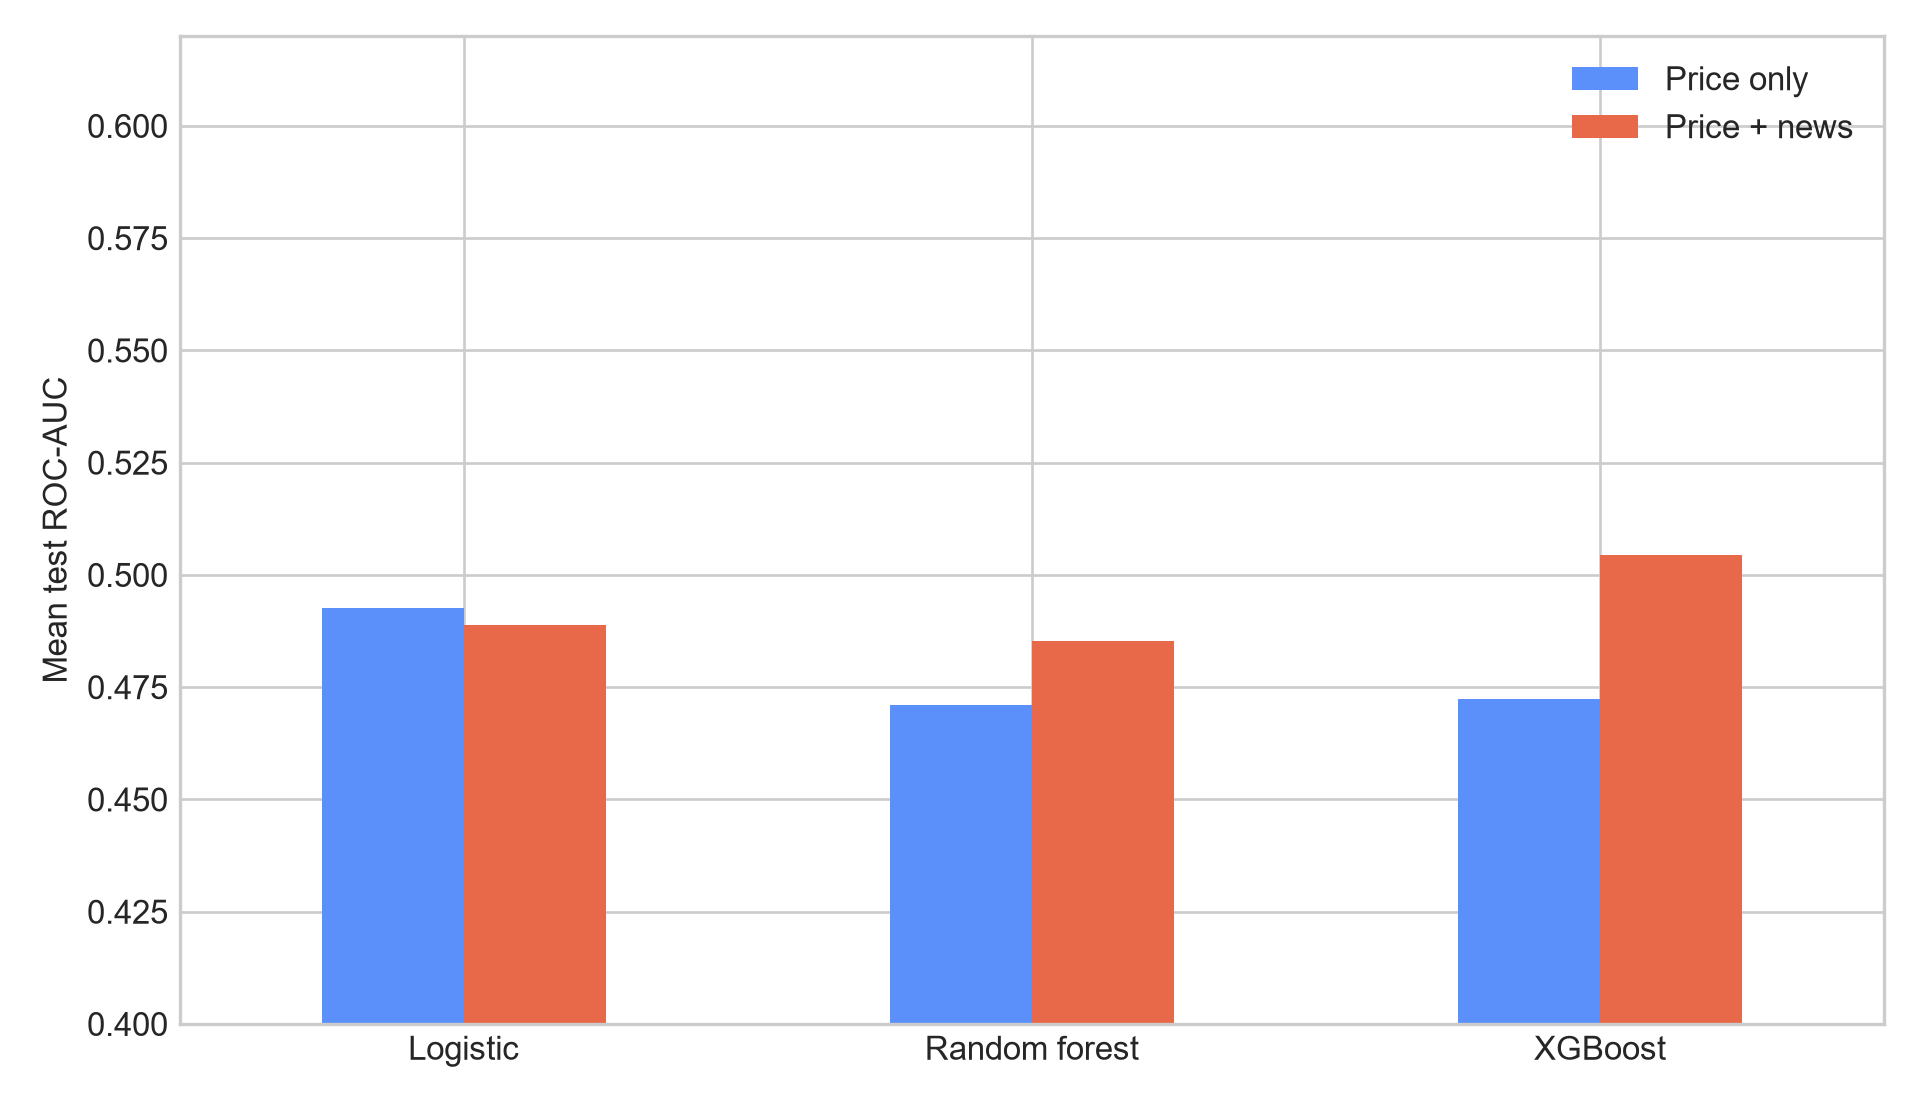
\includegraphics[width=\columnwidth]{figures/model_auc_comparison.png}
\caption{三类模型加入新闻前后的平均测试AUC}
\label{fig:meanauc}
\end{figure}

图\ref{fig:meanauc}还显示模型复杂度并未单调提高表现。价格组中，Logistic反而高于
随机森林和XGBoost，说明量价信号较弱时，复杂模型容易学习历史阶段中的噪声。加入
新闻后，XGBoost改善幅度最大，但绝对AUC仍只有0.504。PR-AUC约0.555主要受上涨类
占比影响，不能被解释为较强预测能力。

\FloatBarrier

\subsection{年度稳定性与显著性}

XGBoost P+N在2014、2015和2016年的AUC分别为0.519、0.533和0.462；P模型分别为
0.518、0.473和0.426。新闻在2015年改善较明显，但2016年两组均低于0.5，H2不成立。
将575个样本外预测合并，AUC增量为0.0348，95\%置信区间为
$[-0.0060,0.0734]$，包含0，故H1仅获得方向性证据，未获得统计显著支持。

\begin{figure}[!htbp]
\centering
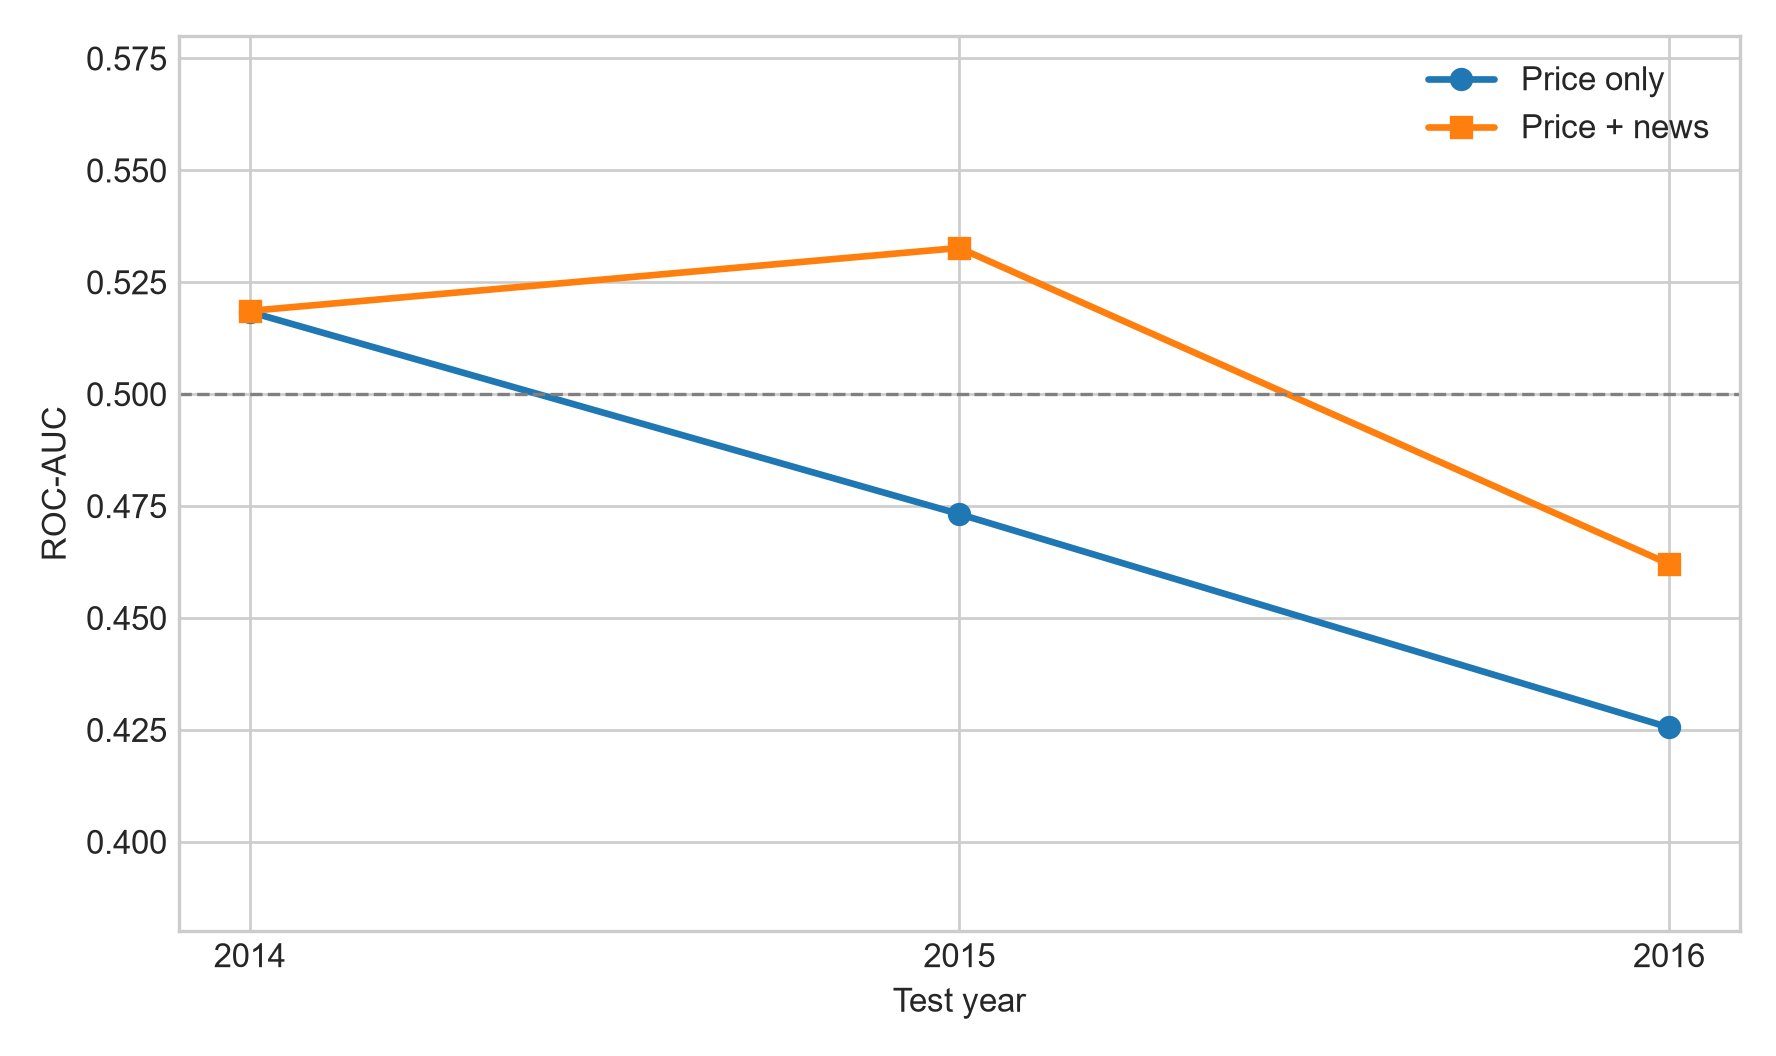
\includegraphics[width=\columnwidth]{figures/yearly_xgboost_auc.png}
\caption{XGBoost仅量价与量价加新闻的逐年AUC}
\label{fig:yearauc}
\end{figure}

2014年两组几乎相同，说明新闻没有明显边际作用；2015年P+N比P高约0.059，是主要
增量来源；2016年P+N虽仍高于P，但两者都低于随机线。由于2016测试样本只有107日，
该结果可能同时包含市场状态变化与小样本波动。总体上，新闻增量方向并非完全相反，
但其绝对预测能力和稳定性不足。

\begin{figure}[!htbp]
\centering
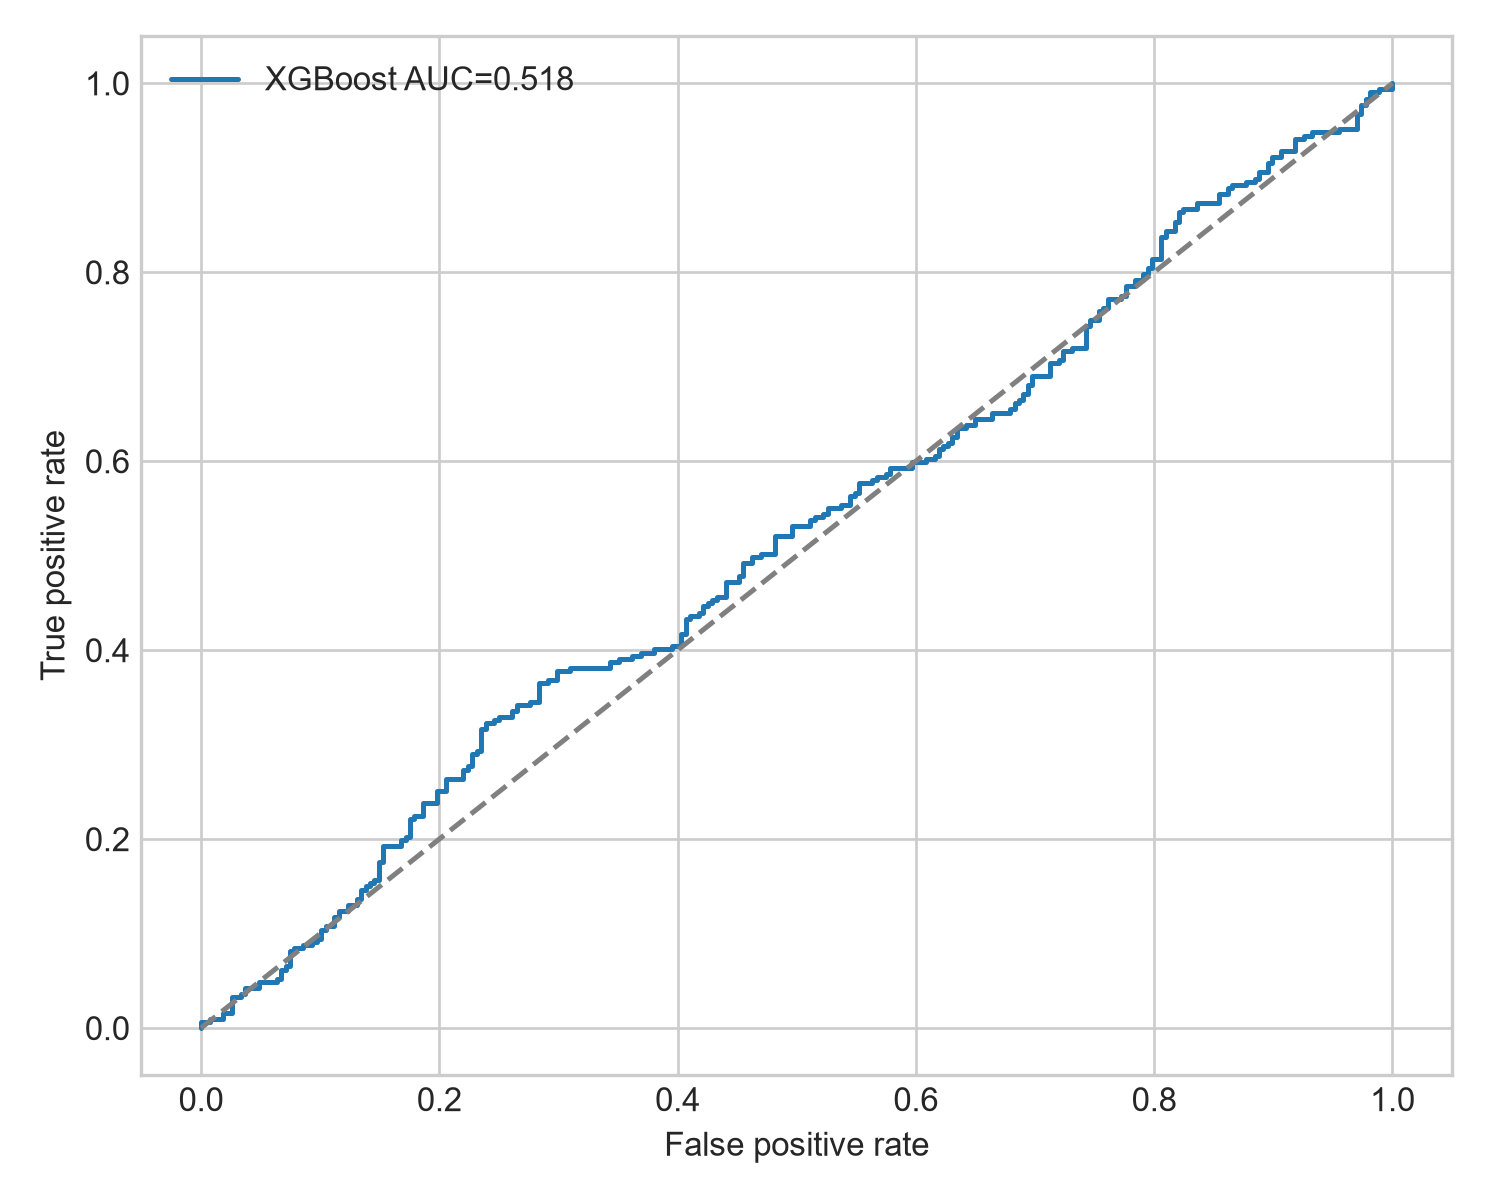
\includegraphics[width=0.90\columnwidth]{figures/xgboost_roc_curve.png}
\caption{XGBoost P+N模型合并测试期ROC曲线}
\label{fig:roc}
\end{figure}

合并测试期ROC-AUC为0.518，高于逐年AUC简单平均0.504，是因为不同年份样本数和
预测分布不同。两者均说明辨别能力较弱，不能将0.5附近的数值解释为稳定优势。

\subsection{错误类型分析}

从各折结果看，验证集选择的F1阈值多位于0.35--0.43，模型倾向预测上涨。以2014年
XGBoost P+N为例，上涨召回率接近0.98，但平衡准确率仅0.489，说明较高F1主要来自
覆盖多数上涨样本，而不是同时识别上涨和下跌。2016年该模型甚至将测试样本几乎全部
判断为上涨，F1达到0.723，平衡准确率却只有0.511。由此可见，在轻度类别不平衡下，
单独使用F1会产生过度乐观的印象。

下跌日通常更难预测。一方面，负面新闻是否造成指数下跌取决于事件是否已经被价格
预期；另一方面，同一宏观事件可能对不同成分股产生相反影响，指数层面会相互抵消。
因此，公司级新闻用于个股横截面预测，理论上比全球新闻用于指数方向预测更有优势。

\FloatBarrier

\subsection{概率校准与阈值敏感性}

分类排序能力并不等于概率可靠。图\ref{fig:calibration}显示各概率分箱的实际上涨
频率围绕理想线明显波动，Brier分数为0.256，略差于无信息概率基准附近水平。
这意味着0.60的预测概率并不稳定对应60\%上涨频率。

\begin{figure}[!htbp]
\centering
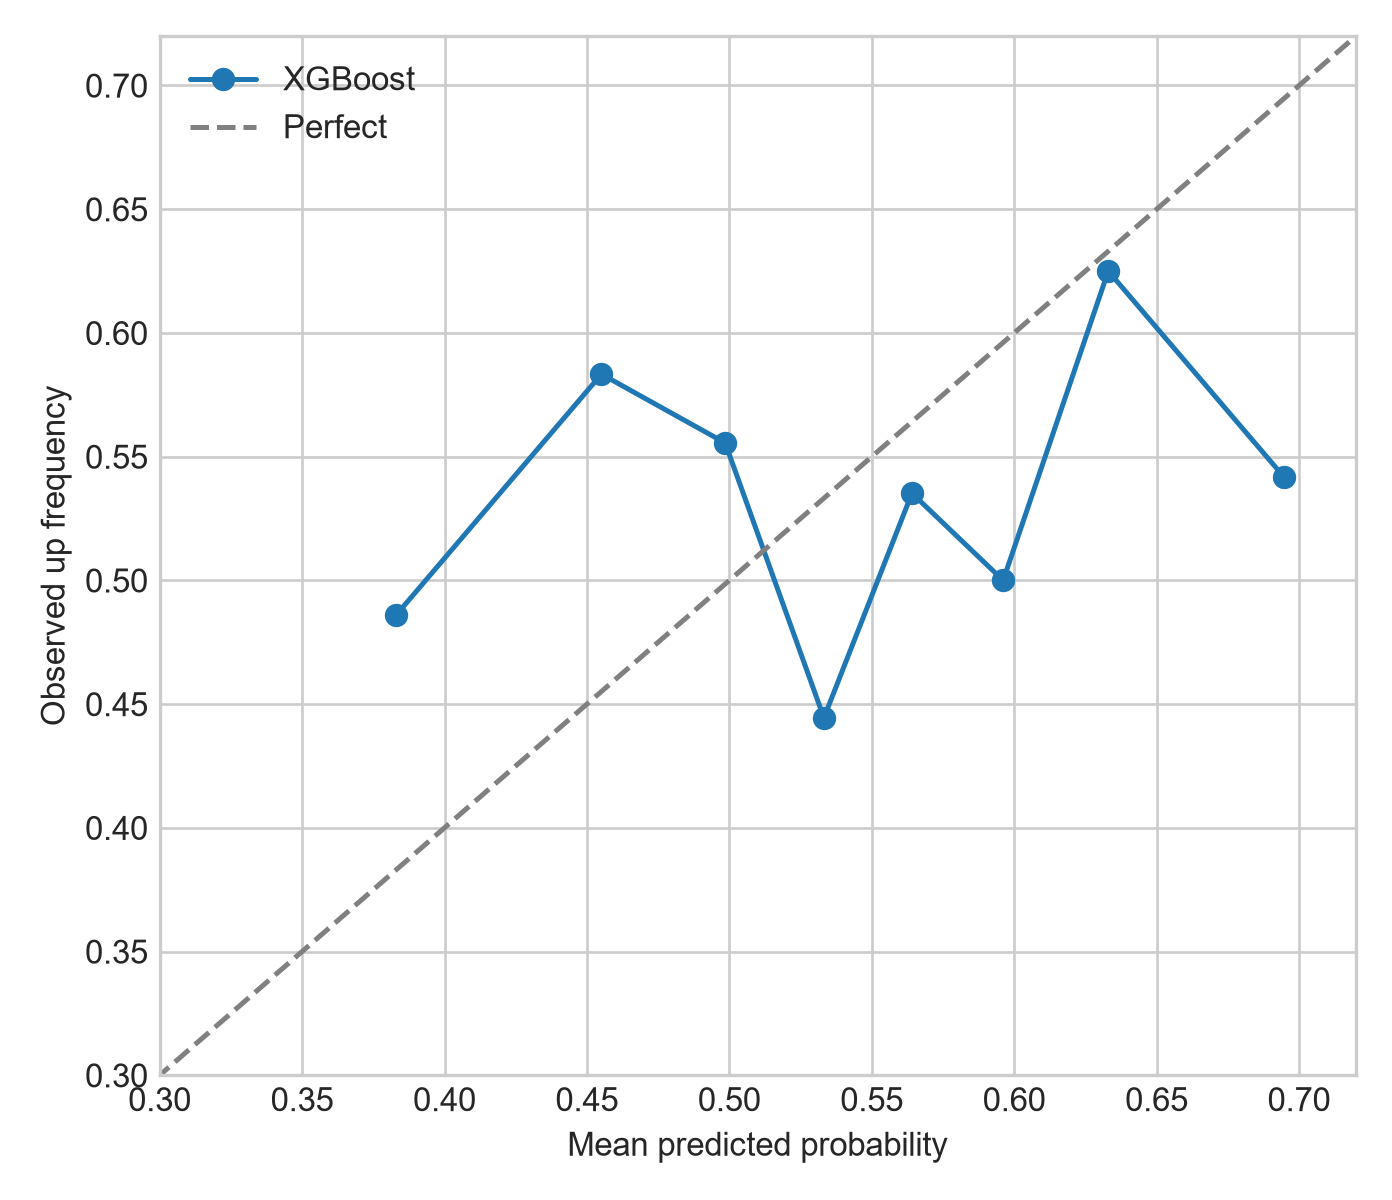
\includegraphics[width=0.94\columnwidth]{figures/calibration_curve.png}
\caption{XGBoost P+N模型的概率校准曲线}
\label{fig:calibration}
\end{figure}

校准图在0.45附近高于理想线、在0.53附近低于理想线，反映预测概率排序与实际频率
并不一致。造成该现象的原因可能是不同年份的基础上涨概率变化，而模型没有进行逐折
Platt scaling或isotonic calibration。若概率将用于仓位管理，校准应当和AUC同等
重要。

阈值从0.40提高到0.65时，年化净收益大幅变化。0.40--0.45附近出现小幅正收益，
但该范围意味着高持仓比例，且阈值0.475之后大多为负。结果对人为阈值高度敏感，
无法支持稳定策略。

\begin{figure}[!htbp]
\centering
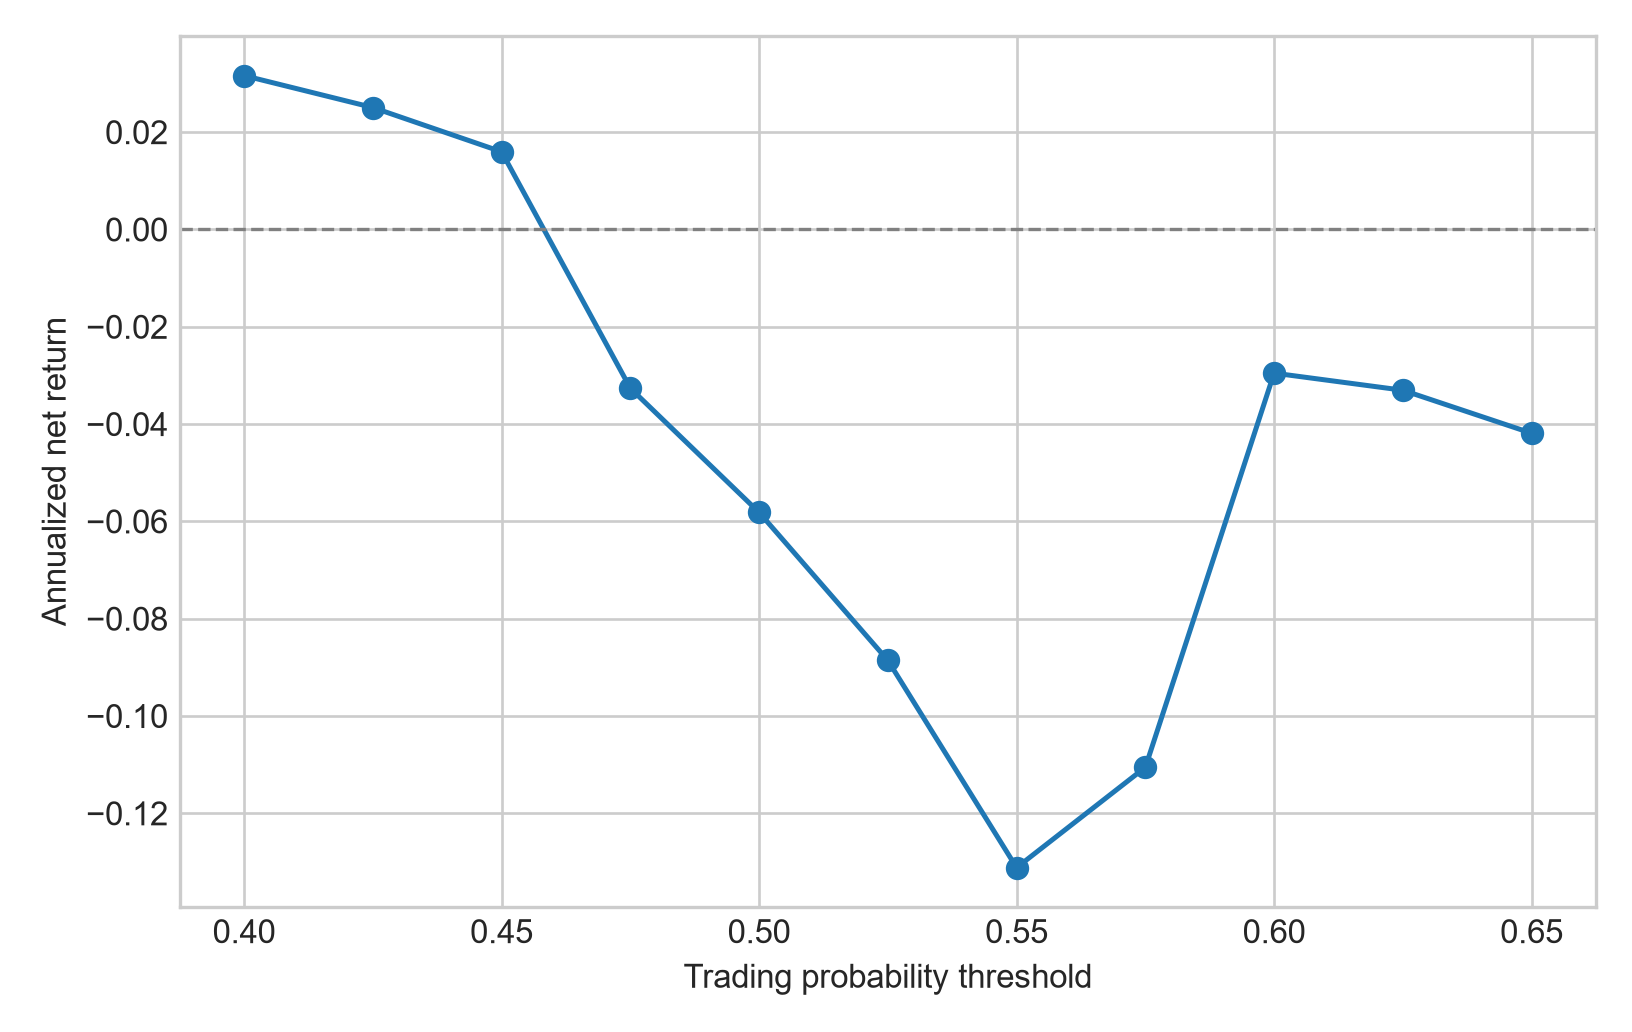
\includegraphics[width=\columnwidth]{figures/threshold_sensitivity.png}
\caption{交易概率阈值与样本外年化净收益}
\label{fig:threshold}
\end{figure}

低阈值策略的少量正收益并不能证明新闻信号有效，因为其仓位接近长期持有，收益主要
可能来自市场上涨漂移。阈值提高后，模型只选择自认为更确定的交易日，但收益反而下降，
进一步表明预测概率没有形成单调的经济排序。

\FloatBarrier

\subsection{经济性结果}

\begin{table}[t]
\centering
\caption{XGBoost新闻策略经济指标}
\small
\begin{tabular}{lr}
\toprule
指标 & 数值\\
\midrule
样本外交易日 & 575\\
持仓比例 & 48.52\%\\
年化净收益 & $-13.12\%$\\
年化波动率 & 8.69\%\\
夏普比率 & $-1.51$\\
最大回撤 & $-29.46\%$\\
DJIA买入持有年化收益 & 8.95\%\\
\bottomrule
\end{tabular}
\label{tab:strategy}
\end{table}

图\ref{fig:return}显示新闻策略从2014年起持续落后，2015年市场波动期间回撤明显。
统计上的微弱排序提升没有转化为经济收益，H3不成立。

\begin{figure}[!htbp]
\centering
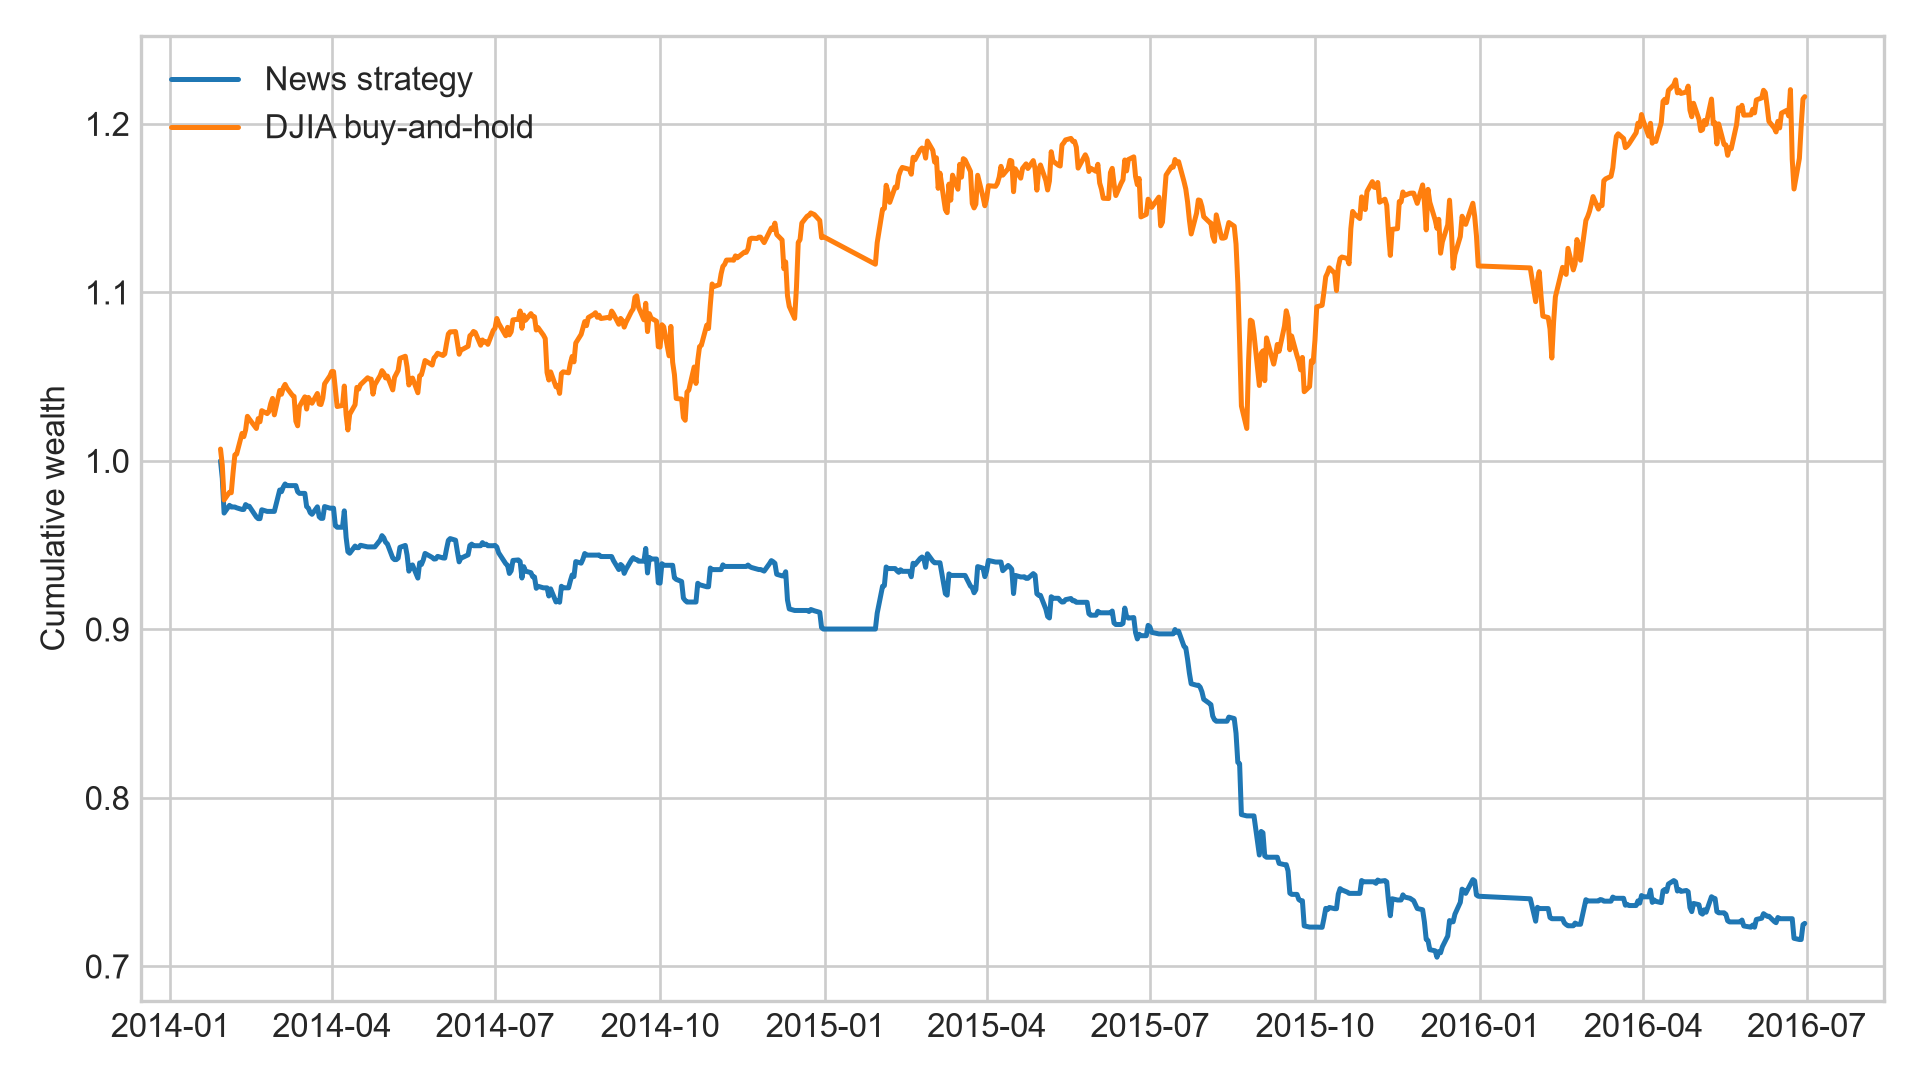
\includegraphics[width=\columnwidth]{figures/cumulative_returns.png}
\caption{新闻策略与DJIA买入持有的样本外累计净值}
\label{fig:return}
\end{figure}

策略只在48.52\%的日期持仓，却承担了持续的信号切换成本。累计净值在2015年8月至
9月附近出现明显下降，此后没有恢复。即使忽略交易成本，模型对上涨日的筛选质量也
不足以弥补空仓期间错过的市场收益。该结果说明，分类指标和资产管理目标之间存在
明显差距：一个略高于0.5的AUC并不意味着能构造盈利策略。

\FloatBarrier

\section{讨论}

\subsection{为什么新闻信号较弱}

第一，标题是Reddit筛选的全球热点，包含战争、政治和社会事件，不完全对应DJIA
成分公司。公司级新闻与个股价格的映射比“全球新闻--指数”映射更直接。第二，
VADER未在金融语料训练，对盈利预警、评级变化和并购条款的理解弱于FinBERT。
第三，日均聚合会抵消同日正负事件，且丢失新闻排序、主体和事件类型。第四，公开
新闻可能快速入价，日频下一日预测窗口过长。第五，市场机制随年份变化，导致
2014--2015的弱信号无法延续至2016。

此外，情绪方向与价格方向之间不是简单的一一对应关系。负面宏观新闻可能促使市场
预期宽松政策，从而产生反向价格反应；已经被充分预期的利空公布后，价格也可能出现
“利空出尽”。VADER只判断语言语调，无法区分事件是否超出市场预期，更无法识别
新闻相对于分析师预测的惊喜程度。因此，情绪分数与收益相关性接近零并不意味着新闻
完全无用，而是说明“语调”不足以替代“事件与预期差”。

新闻聚合方式也会造成信息损失。每日25条标题中，某一条高影响政策新闻可能远比其他
24条重要，但等权平均会将其稀释。相反，多条描述同一事件的标题可能被重复计数。
更完善的系统应进行事件聚类、来源去重和重要性加权，再将公司、行业和宏观事件分别
建模。

\subsection{与既有研究的关系}

本文结果并不否定新闻文本的研究价值，而是界定了低粒度数据和简单情绪聚合的边界。
Ding等的事件表示保留主体与动作\cite{ding2015}，StockNet保留文本序列和价格动态
\cite{stocknet}，FinBERT提供金融领域语义\cite{finbert}，FNSPID与CausalStock
提供公司级大样本和关系信息\cite{fnspid,causalstock}。相比之下，本研究更接近
一个严格验证的教学基线。其价值在于说明：若没有精确时间戳、公司映射和更丰富文本
表示，增加复杂分类器并不能自动获得可交易信号。

\subsection{非显著结果的研究价值}

金融预测存在较强的结果发表偏差，表现较好的模型更容易被展示，而接近随机或回测
失败的结果较少被讨论。本文的非显著结果提供两点启示。第一，采用随机划分或同日
标签可能会得到更漂亮的数字，但这些数字不一定能代表部署效果。第二，模型选择不能
替代数据质量。即使XGBoost能够拟合复杂关系，如果新闻与预测对象的映射本身较弱，
模型只会在有限样本中寻找不稳定模式。

从教学角度，拒绝H1--H3并不等于实验失败。研究假设的作用是形成可证伪问题，
而不是保证得到正向结论。只要数据处理透明、验证流程合理、结论与证据一致，负结果
同样能够回答研究问题，并为下一步改进提供方向。

\section{应用意义与系统设计启示}

\subsection{在智能投研中的合理定位}

根据本实验，新闻情绪不适合单独作为自动交易开关，但可以作为投研系统的辅助变量。
例如，当新闻负面占比和波动率同时升高时，系统可以提高风险提示等级；当情绪模型
识别到极端事件时，可将相关日期推送给分析师复核。这样的“人机协同”场景不要求
情绪分数直接预测收益，而强调信息筛选、异常发现和解释支持。

若用于真实产品，系统至少应分为四层：数据层负责接入带时间戳的新闻与行情；NLP层
完成公司实体识别、事件分类和金融情绪分析；预测层融合文本、量价和市场状态；
评价层持续监控AUC、校准、漂移和交易成本。模型输出应包含置信度和主要影响变量，
而不是只给出“买入/卖出”的黑箱结论。

\subsection{风险控制要求}

金融模型容易受到概念漂移影响。政策环境、市场参与者和新闻传播速度会不断变化，
历史关系可能在未来失效。因此上线系统应采用滚动训练、时间外监控和失效阈值。
当AUC连续多个窗口低于0.5、概率校准明显偏离或交易回撤超过限制时，应暂停信号，
而不是继续根据历史最优参数运行。

数据合规同样重要。新闻全文可能受版权限制，商业系统需要确认授权范围；用户界面
应明确模型不构成投资建议；回测结果必须说明样本区间、成本假设和幸存者偏差。
这些要求决定了金融AI产品不仅是模型问题，也包含数据治理和风险披露。

\section{稳健性、局限与扩展}

本文已完成三类稳健性诊断：逐年AUC比较、bootstrap置信区间、不同交易阈值回测。
结果均指向信号不稳定。仍有以下局限：
\begin{enumerate}
  \item 新闻缺少精确发布时间，无法区分盘前、盘中和盘后；
  \item 样本仅约2000日，2016测试期只有上半年；
  \item VADER不是金融领域模型，且未利用完整文本；
  \item 回测使用DJIA指数收益，未包含滑点与实际产品跟踪误差；
  \item 固定超参数减少了数据窥探，但可能不是每折最优参数。
\end{enumerate}

后续研究应优先改进数据而非盲目堆叠模型：使用FNSPID等带时间戳和股票代码的数据；
以FinBERT或Financial PhraseBank微调模型提取情绪；保留新闻来源、排名、主体和
事件类别；分别预测盘前到收盘、收盘到次日开盘等窗口；使用历史指数成分和行业关系；
以超过交易成本的收益阈值构造标签；采用概率校准及purged/embargo验证。

\subsection{建议的扩展实验}

第一，比较VADER、Loughran--McDonald词典与FinBERT。三种方法分别代表通用规则、
金融词典和领域预训练模型，可以判断提升来自更好的金融语义还是更复杂的预测器。
第二，对Top1--Top5与Top6--Top25分别聚合，以检验新闻排名是否包含注意力信息。
第三，将标签改为收益率超过$\pm0.2\%$的三分类任务，减少微小随机波动对标签的影响。
第四，在高波动和低波动状态下分别训练模型，检验新闻价值是否具有市场状态依赖。
第五，使用TF--IDF加Logistic回归建立直接文本基线，避免情绪聚合丢失主题信息。

这些扩展应继续遵守相同的时间划分，不能在看到测试结果后反复修改阈值。若进行多组
实验，还需要报告全部方案或进行多重检验调整，避免只保留偶然表现最好的组合。

\section{可复现性说明}

实验代码采用固定随机种子42。原始数据保存为两个CSV文件：每日新闻标题表和DJIA
行情表。脚本依次执行文本清洗、VADER推理、日度聚合、量价特征计算、下一日标签
构造、walk-forward训练、bootstrap、回测和绘图。输出包括模型面板Parquet、
逐折指标CSV、预测概率Parquet、每日策略收益CSV以及诊断JSON。

主要软件环境为Python、Pandas、NumPy、scikit-learn、XGBoost、VADER Sentiment、
Matplotlib和PyArrow。所有模型参数和特征名均写入脚本，图表直接由真实输出生成。
复现实验时运行\texttt{code/djia\_experiment.py}，并分别传入新闻CSV、行情CSV和
输出目录参数。生成的
\texttt{metrics\_summary.csv}对应表\ref{tab:result}，
\texttt{diagnostics.json}记录bootstrap与回测结果。论文没有使用模拟数据或手工
修改图表数值。

\FloatBarrier

\section{结论}

本文以1968个交易日和49193条标题构建了新闻情绪与DJIA量价融合的下一日方向预测。
严格walk-forward结果显示，XGBoost加入新闻后平均AUC由0.472提高至0.504，但
bootstrap置信区间包含0；逐年表现不稳定，概率校准较差，0.55阈值策略年化收益
$-13.1\%$。因此，该数据和VADER聚合方法至多提供微弱、时变的非线性信息，不足以
支持稳定预测或交易应用。研究说明，金融机器学习中时间对齐、样本外验证和经济检验
比单纯提高模型复杂度更重要。

总体而言，本研究完成了从数据获取、文本量化、异构融合、时序验证到经济检验的完整
流程。最重要的发现不是某个模型取得了高准确率，而是新闻增量在严格验证下十分有限。
这为后续研究设定了清晰基线：只有当更精确的时间戳、公司级映射和金融领域文本表示
能够稳定超过本文结果，并在交易成本后保持有效，才能认为新闻驱动预测具有实际价值。

\begin{thebibliography}{99}\scriptsize
\bibitem{tetlock}
Tetlock, P. C. Giving Content to Investor Sentiment: The Role of Media in the Stock Market.
\emph{The Journal of Finance}, 62(3):1139--1168, 2007.

\bibitem{lm}
Loughran, T., McDonald, B. When Is a Liability Not a Liability? Textual Analysis,
Dictionaries, and 10-Ks. \emph{The Journal of Finance}, 66(1):35--65, 2011.

\bibitem{phrasebank}
Malo, P., Sinha, A., Korhonen, P., Wallenius, J., Takala, P.
Good Debt or Bad Debt: Detecting Semantic Orientations in Economic Texts.
\emph{JASIST}, 65(4):782--796, 2014.

\bibitem{vader}
Hutto, C. J., Gilbert, E. VADER: A Parsimonious Rule-based Model for Sentiment
Analysis of Social Media Text. \emph{ICWSM}, 2014.

\bibitem{ding2015}
Ding, X., Zhang, Y., Liu, T., Duan, J. Deep Learning for Event-Driven Stock Prediction.
\emph{IJCAI}, 2015.

\bibitem{stocknet}
Xu, Y., Cohen, S. B. Stock Movement Prediction from Tweets and Historical Prices.
\emph{ACL}, 2018.

\bibitem{akita}
Akita, R., Yoshihara, A., Matsubara, T., Uehara, K.
Deep Learning for Stock Prediction Using Numerical and Textual Information.
\emph{IEEE/ACIS ICIS}, 2016.

\bibitem{finbert}
Araci, D. FinBERT: Financial Sentiment Analysis with Pre-trained Language Models.
arXiv:1908.10063, 2019.

\bibitem{fnspid}
Dong, Z., Fan, X., Peng, Z. FNSPID: A Comprehensive Financial News Dataset in Time Series.
arXiv:2402.06698, 2024.

\bibitem{causalstock}
Soun, Y., et al. CausalStock: Deep End-to-end Causal Discovery for News-driven
Stock Movement Prediction. \emph{NeurIPS}, 2024.

\bibitem{rf}
Breiman, L. Random Forests. \emph{Machine Learning}, 45:5--32, 2001.

\bibitem{xgboost}
Chen, T., Guestrin, C. XGBoost: A Scalable Tree Boosting System.
\emph{KDD}, 785--794, 2016.

\bibitem{lop}
L\'opez de Prado, M. \emph{Advances in Financial Machine Learning}. Wiley, 2018.

\bibitem{dataset}
Sun, J. Daily News for Stock Market Prediction, Version 1. Kaggle, 2016.
\url{https://www.kaggle.com/datasets/aaron7sun/stocknews}.
\end{thebibliography}

\end{document}
